\documentclass[11pt]{article}
\usepackage[margin=1in]{geometry}
\usepackage[T1]{fontenc}
\usepackage{amsmath,amssymb,amsthm}
\usepackage[hidelinks]{hyperref}
\usepackage{graphicx}

\newtheorem{theorem}{Theorem}
\newtheorem{lemma}{Lemma}
\newtheorem{remark}{Remark}

\DeclareMathOperator{\PiOne}{\Pi_1}

\title{A Proof of the Dominated Bilinear Forms Tensor Conjecture}
\author{FA Banach run: \texttt{fa\_banach\_001}}
\date{2026-06-28}

\begin{document}
\maketitle

\section*{Source Problem}

The source paper is:
\begin{quote}
G. Botelho, D. Pellegrino, and P. Rueda,
\emph{Dominated bilinear forms and 2-homogeneous polynomials},
arXiv:0905.2079.
\end{quote}

The final conjecture of the paper asks whether, for an infinite-dimensional
Banach space \(X\),
\[
  \mathcal L_{d,1}({}^2X)=\mathcal L({}^2X)
  \quad\Longrightarrow\quad
  X\widehat\otimes_\pi X=X\widehat\otimes_\varepsilon X .
\]
Here \(\mathcal L_{d,1}({}^2X)\) denotes the continuous scalar-valued bilinear
forms on \(X\times X\) which are \(1\)-dominated.

\begin{center}
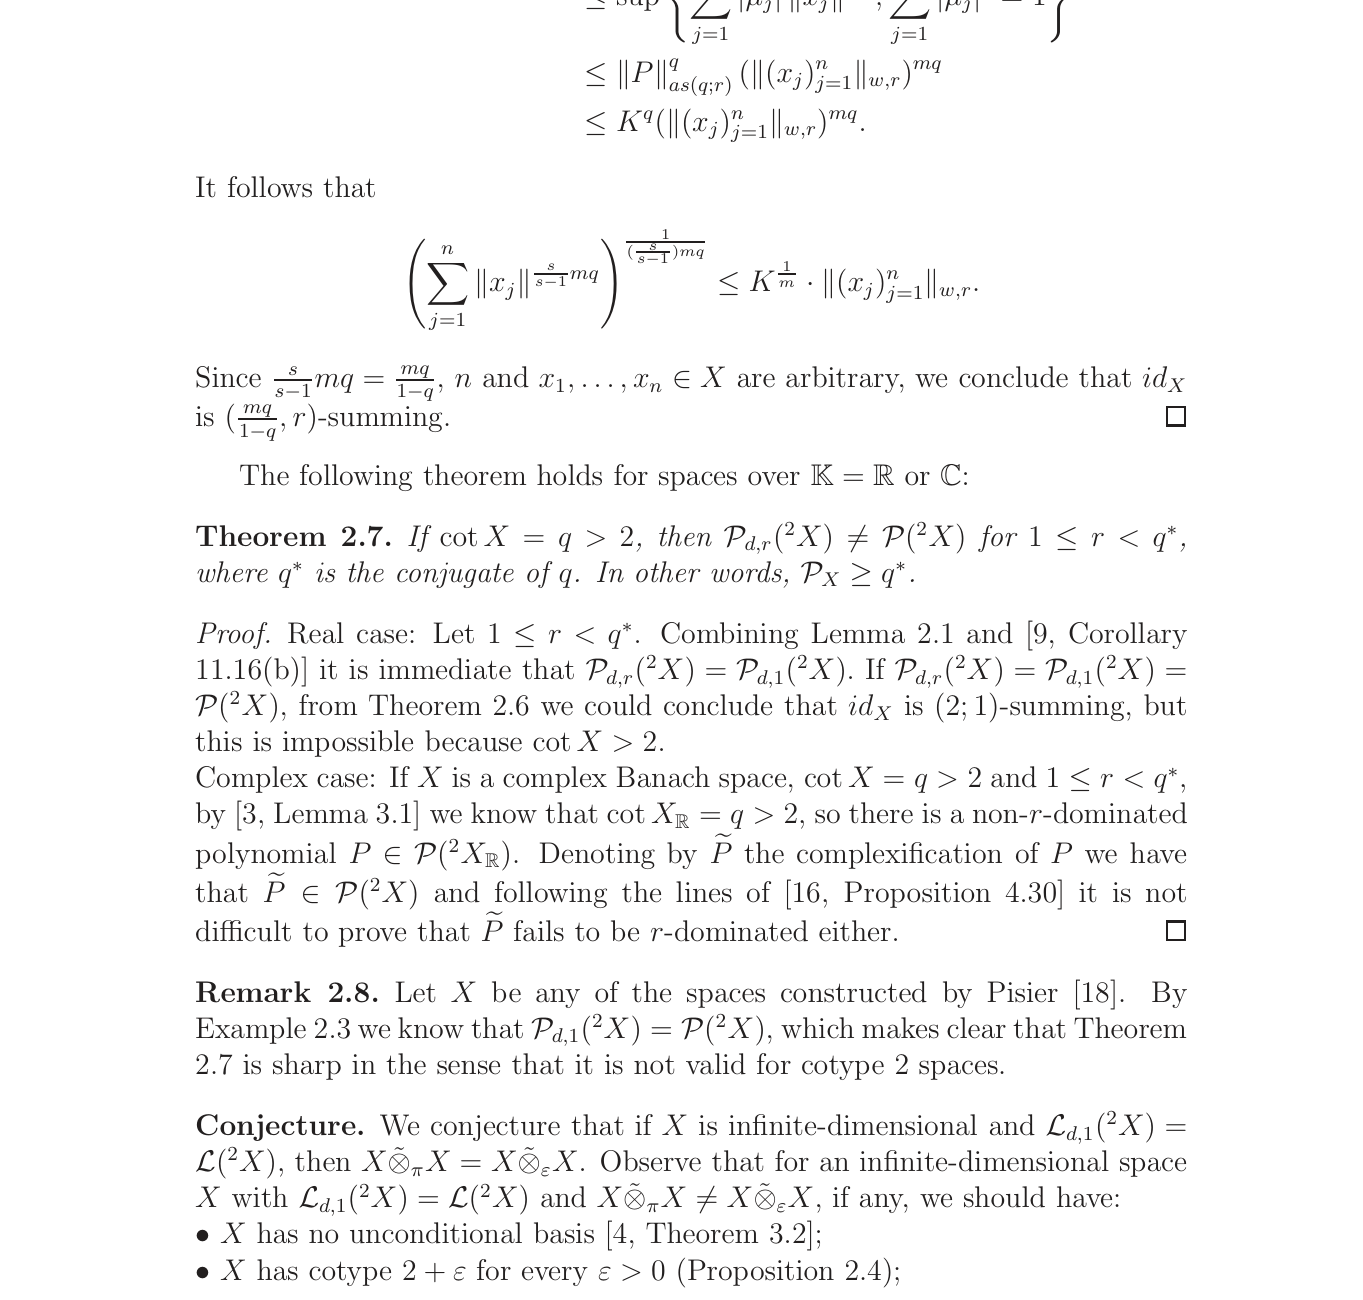
\includegraphics[width=0.92\textwidth]{figures/open_problem_crop_page6.png}

\vspace{0.5em}

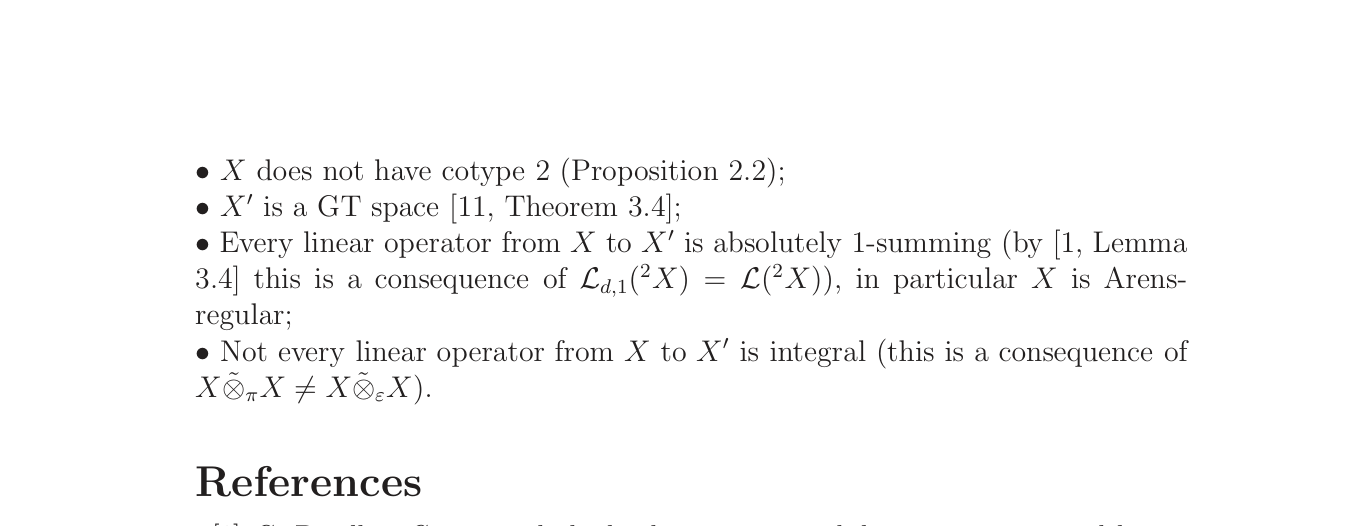
\includegraphics[width=0.92\textwidth]{figures/open_problem_crop_page7.png}
\end{center}

\section*{Result}

\begin{theorem}
Let \(X\) be a Banach space. If every continuous scalar-valued bilinear form on
\(X\times X\) is \(1\)-dominated, then every continuous scalar-valued bilinear
form on \(X\times X\) is integral. Consequently
\[
  X\widehat\otimes_\pi X=X\widehat\otimes_\varepsilon X .
\]
In particular, the conjecture from arXiv:0905.2079 is true. The
infinite-dimensional hypothesis is not needed.
\end{theorem}

\section*{Proof Intuition}

The obstruction listed in the source paper says that a counterexample would
have an operator \(T:X\to X^*\) which is not integral. We show that this cannot
happen.

The hypothesis first implies that every operator \(X\to X^*\) is absolutely
\(1\)-summing. This is already noted in the source paper, but the proof is
short and is included below. The missing point is to make the adjoint
\[
T^*:X^{**}\to X^*
\]
absolutely \(1\)-summing as well, because the standard duality theorem for
integral operators says that \(T\) is integral exactly when \(T^*\) is
\(1\)-summing.

To prove this adjoint estimate, one uses local reflexivity. A finite family in
\(X^{**}\) can be pulled back almost isometrically to \(X\) while preserving its
values on finitely many functionals of the form \(Tx\). The orientation matters:
the estimate uses the transposed operator \(T^\tau(y)(x)=T(x)(y)\), which is
also absolutely \(1\)-summing because the hypothesis applies to the transposed
bilinear form.

\section*{Definitions and Standard Facts}

For a finite sequence \((x_j)_{j=1}^n\) in \(X\), write
\[
\|(x_j)_{j=1}^n\|_{w,1}
  =\sup_{x^*\in B_{X^*}}\sum_{j=1}^n |x^*(x_j)|.
\]
A bilinear form \(A:X\times X\to\mathbb K\) is \(1\)-dominated if there is a
constant \(D\) such that, for all finite sequences \((x_j)\) and \((y_j)\) in
\(X\),
\[
\left(\sum_{j=1}^n |A(x_j,y_j)|^{1/2}\right)^2
\le D\,\|(x_j)_{j=1}^n\|_{w,1}\,\|(y_j)_{j=1}^n\|_{w,1}.
\tag{1}
\]

We use two standard facts. First, the principle of local reflexivity: if
\(E\subset X^{**}\) and \(F\subset X^*\) are finite-dimensional and
\(\delta>0\), then there is a linear map \(R:E\to X\) with
\(\|R\|\le 1+\delta\) such that
\[
  f(Rx^{**})=x^{**}(f)\qquad(x^{**}\in E,\ f\in F).
\]
Second, the duality theorem for integral operators:
\[
  T:X\to Y \text{ is integral }
  \quad\Longleftrightarrow\quad
  T^*:Y^*\to X^* \text{ is absolutely }1\text{-summing}.
\tag{2}
\]
We cite these in the standard forms found in the literature on tensor norms
and absolutely summing operators.

\section*{From Dominated Bilinear Forms to Summing Operators}

\begin{lemma}
Let \(T:X\to X^*\) be bounded and set \(A_T(x,y)=T(x)(y)\). If \(A_T\) is
\(1\)-dominated, then \(T\) is absolutely \(1\)-summing.
\end{lemma}

\begin{proof}
Let \(D\) be a constant for \(A_T\) in (1). Fix \(x_1,\ldots,x_n\in X\) and
\(\eta>0\). Choose \(y_j\in B_X\) so that
\[
  |T(x_j)(y_j)|\ge (1-\eta)\|T x_j\|.
\]
Put \(a_j=|T(x_j)(y_j)|\). If \(\sum_j a_j=0\), there is nothing to prove.
Otherwise apply (1) to the two sequences \((x_j)\) and \((a_j y_j)\). Since
\[
  \|(a_j y_j)_{j=1}^n\|_{w,1}
  \le \sum_{j=1}^n a_j,
\]
we get
\[
\left(\sum_{j=1}^n |a_j T(x_j)(y_j)|^{1/2}\right)^2
\le
D\,\|(x_j)_{j=1}^n\|_{w,1}\sum_{j=1}^n a_j .
\]
The left side is \((\sum_j a_j)^2\). Cancelling \(\sum_j a_j\) gives
\[
  \sum_{j=1}^n a_j
  \le D\,\|(x_j)_{j=1}^n\|_{w,1}.
\]
Letting \(\eta\downarrow0\), we obtain
\[
  \sum_{j=1}^n \|T x_j\|
  \le D\,\|(x_j)_{j=1}^n\|_{w,1}.
\]
Thus \(T\) is absolutely \(1\)-summing.
\end{proof}

\section*{The Local Reflexivity Step}

\begin{lemma}
Assume every continuous bilinear form on \(X\times X\) is \(1\)-dominated.
Then, for every bounded operator \(T:X\to X^*\), the adjoint
\[
T^*:X^{**}\to X^*
\]
is absolutely \(1\)-summing.
\end{lemma}

\begin{proof}
Let \(T:X\to X^*\) be bounded. Define the transposed operator
\[
  T^\tau:X\to X^*,\qquad T^\tau(y)(x)=T(x)(y).
\]
The bilinear form associated with \(T^\tau\) is the transpose of \(A_T\), so it
is \(1\)-dominated by hypothesis. By the preceding lemma, \(T^\tau\) is
absolutely \(1\)-summing.

Let \(x_1^{**},\ldots,x_n^{**}\in X^{**}\) and let \(\eta>0\). Choose
\(z_j\in B_X\) such that
\[
  \|T^*x_j^{**}\|
  \le |(T^*x_j^{**})(z_j)|+\eta/n
  = |x_j^{**}(Tz_j)|+\eta/n .
\]
Set
\[
  E=\operatorname{span}\{x_1^{**},\ldots,x_n^{**}\}\subset X^{**},
  \qquad
  F=\operatorname{span}\{Tz_1,\ldots,Tz_n\}\subset X^* .
\]
By local reflexivity, for every \(\delta>0\) there is a linear map
\(R:E\to X\) with \(\|R\|\le1+\delta\) and
\[
  f(Rx^{**})=x^{**}(f)\qquad(x^{**}\in E,\ f\in F).
\]
In particular,
\[
  x_j^{**}(Tz_j)=(Tz_j)(Rx_j^{**})
  =T^\tau(Rx_j^{**})(z_j).
\]
Therefore
\begin{align*}
\sum_{j=1}^n \|T^*x_j^{**}\|
&\le
\eta+\sum_{j=1}^n |T^\tau(Rx_j^{**})(z_j)|\\
&\le
\eta+\sum_{j=1}^n \|T^\tau(Rx_j^{**})\|\\
&\le
\eta+\pi_1(T^\tau)
  \sup_{x^*\in B_{X^*}}\sum_{j=1}^n |x^*(Rx_j^{**})|\\
&\le
\eta+\pi_1(T^\tau)(1+\delta)
  \sup_{\psi\in B_{E^*}}\sum_{j=1}^n |\psi(x_j^{**})|\\
&=
\eta+\pi_1(T^\tau)(1+\delta)
  \|(x_j^{**})_{j=1}^n\|_{w,1}.
\end{align*}
Letting \(\eta\downarrow0\) and \(\delta\downarrow0\) gives
\[
  \sum_{j=1}^n \|T^*x_j^{**}\|
  \le
  \pi_1(T^\tau)\,\|(x_j^{**})_{j=1}^n\|_{w,1}.
\]
Thus \(T^*\) is absolutely \(1\)-summing.
\end{proof}

\section*{Proof of the Theorem}

Let \(A:X\times X\to\mathbb K\) be a continuous bilinear form, and let
\[
  T_A:X\to X^*,\qquad T_A(x)(y)=A(x,y),
\]
be its associated operator. By the local reflexivity lemma,
\[
  T_A^*:X^{**}\to X^*
\]
is absolutely \(1\)-summing. By the integral-operator duality (2), \(T_A\) is
integral. Equivalently, \(A\) is an integral bilinear form.

Hence every continuous scalar-valued bilinear form on \(X\times X\) is
integral. By the standard tensor-norm characterization of integral bilinear
forms, this is equivalent to the identity map on the algebraic tensor product
extending to an isomorphism
\[
  X\widehat\otimes_\pi X \cong X\widehat\otimes_\varepsilon X
\]
given by the canonical tensor identification. In the notation of the source
paper,
\[
  X\widehat\otimes_\pi X=X\widehat\otimes_\varepsilon X .
\]
This proves the conjecture.

\section*{Verification Notes}

The proof is non-computational. The only delicate point is the orientation in
the local-reflexivity argument: \(x^{**}(Tz)\) is represented as
\((Tz)(Rx^{**})\), which is controlled by the transposed operator
\(T^\tau\), not by \(T\). Since the hypothesis applies to all bilinear forms,
\(T^\tau\) is absolutely \(1\)-summing by the first lemma.

The argument does not use infinite dimensionality, cotype, unconditionality, or
any approximation property.

\section*{Novelty Check}

On 2026-06-28, I checked the lightweight run indexes for arXiv:0905.2079,
``dominated bilinear'', ``2-homogeneous'', and the tensor-product keywords.
No prior packet or attempt for this conjecture was found. I also searched the
local parsed arXiv source pool for the exact title and close dominated-bilinear
phrases; this found only the source paper and the deterministic scan record.

Web searches on the same date included exact and close variants such as
``all bilinear forms 1-dominated Banach space'', ``Dominated bilinear forms and
2-homogeneous polynomials conjecture'', ``T:X to X* is 1-summing then T is
integral'', and ``absolutely 1-summing X* local reflexivity''. No later explicit
solution of the conjecture was found in that bounded search.

\section*{Human Review Recommendation}

This should be reviewed as a candidate full solution. The main check is the
standard operator-ideal step \(T\) integral iff \(T^*\) is absolutely
\(1\)-summing, and the local-reflexivity estimate showing that \(T^*\) is
\(1\)-summing using \(T^\tau\).

\section*{References}

\begin{thebibliography}{9}
\bibitem{BPR}
G. Botelho, D. Pellegrino, and P. Rueda,
\emph{Dominated bilinear forms and 2-homogeneous polynomials},
arXiv:0905.2079.

\bibitem{DF}
A. Defant and K. Floret,
\emph{Tensor Norms and Operator Ideals},
North-Holland Mathematics Studies 176, North-Holland, 1993.

\bibitem{DJT}
J. Diestel, H. Jarchow, and A. Tonge,
\emph{Absolutely Summing Operators},
Cambridge University Press, 1995.
\end{thebibliography}

\end{document}
